\section{ML Model Results}
\label{sec:results_ML}
In this section we present the results of the ML models we have trained. We then deeply inspect the best performing model, 
in order to understand its features and its performance.


% --------------- Model Selection ---------------

\subsection{Model Selection}
\label{subsec:results_ML_model_selection}

% MATTEO
% - Matrix plot of stepwise (which is results of algorithm 1) for each model --> to justify the chosen features
\subsubsection*{Features Selection}

% CRISTIAN
% - Comparison for each model of the selected parameters --> to justify the chosen parameters
\subsubsection*{Hyperparameters Selection}


% ANDREA
% - Comparison of the three models with best combination of features and best parameters
	% - precision, recall, AUC, accuracy
\subsubsection*{Model Comparison} \label{subsubsec:results_ML_model_comparison}

As depicted in Figure \ref{fig:ML_operative_flow}, we now have six different models: three with only symptoms 
and three with both symptoms and new features. The best model was selected from each group based on their accuracy 
values. Figures \ref{fig:acc_symptoms} and \ref{fig:acc_new_features} indicate consistently low overfitting 
and similar performance across all models in both groups. Despite their varying complexity, the models achieve 
similar performance on the test set, meaning that a linear separation boundary is sufficient to properly classify
the features vector. This founds justification in the highly discriminative nature of the features of this dataset.

\begin{figure}[H]
	\centering
	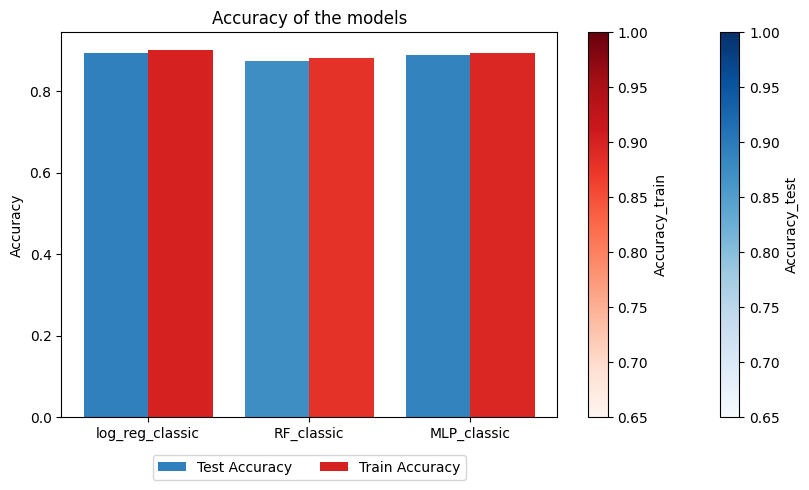
\includegraphics[width=\columnwidth]{images/acc_symptoms.png}
	\caption{Accuracy of the three models with only symptoms}
	\label{fig:acc_symptoms}
\end{figure}

\begin{figure}[H]
	\centering
	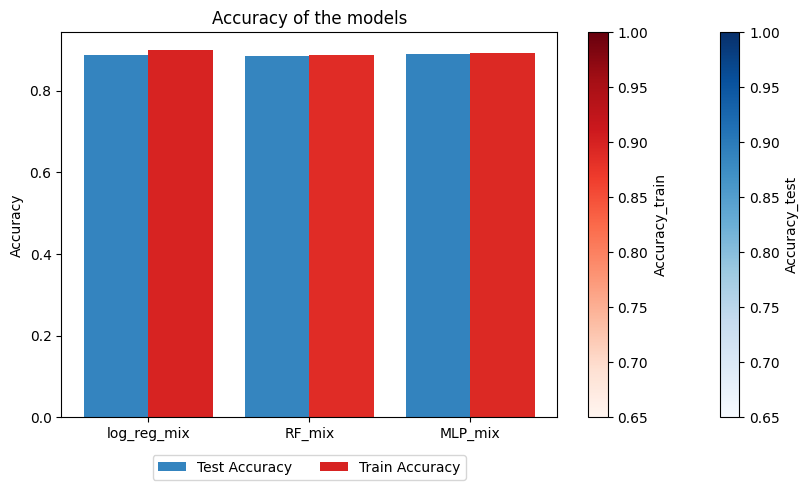
\includegraphics[width=\columnwidth]{images/acc_new_features.png}
	\caption{Accuracy of the three models with new features}
	\label{fig:acc_new_features}
\end{figure}



% --------------- New Features Effect ---------------

\subsection{New Features Effect}
% ANDREA
% - compare the best symptoms one hot model with the best one with the new features

\noindent
The best model from each group was further trained on the full balanced dataset to ensure a more reliable 
performance evaluation. The results in Figure \ref{fig:acc_best_models} reveal a minimal difference between 
the two groups. This addresses our \textbf{first goal}: the new features, while not improving the model, 
offer a comparable performance to using symptoms alone. However, It's essential to note that the new features are 
more numerous than the symptoms, contributing to a more complex model. In conclusion, the extracted network 
features are not a superior alternative to symptoms. 

It is noteworthy that the 'simplicity' of the dataset, leads to a very high accuracy in all models, thus may also affect the performance
evaluation of the new features, which have a small room to improve the model. Therefore, a possible avenue
for future exploration could involve the use of more complex dataset, to better assess the performance of the
new features.

Another viable option for future work is to use the new features as a complement to the symptoms.


% THE FIGURE IS THE FIGURE OF MODEL FULLY TRAINED ON THE BALANCED DATASET


\begin{figure}[H]
	\centering
	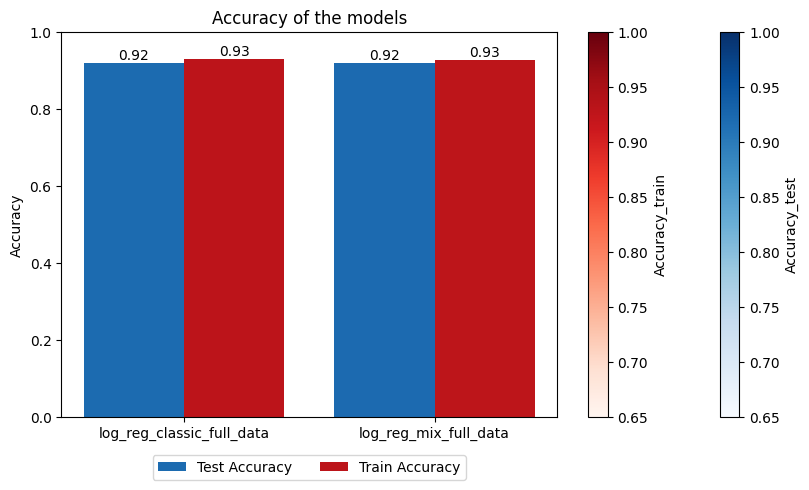
\includegraphics[width=\columnwidth]{images/acc_best_models.png}
	\caption{Accuracy of the best models from both groups}
	\label{fig:acc_best_models}
\end{figure}



% --------------- Best Model Performance ---------------

\subsection{Best Model Analysis}
% DAVIDE
% - what are its features
% - confusion matrix computed on the 4 class diseases (HighL1 - HighL2, LowL1 - HighL2, ...)
% - Worst error
% - Most impactful symptoms



\subsection{Computational Complexity}
% MATTEO
% - apply the reduction technique based on symptoms importance (L1 and L2 combined in the 4 classes)
% - compare the performance of the reduced model with the original one
	% - precision, recall, AUC, accuracy
% - compare the times needed to train the two models


% CRISTIAN
% - 6 Modelli: 3 con solo sintomi, 3 con nuove features
% - - Salvati (joblib) 
% - - Tempo di training

